\section{Design}

\subsection{Introduction}

The design chapter goes through the various design choices. It explains the architecture and components among other aspects. At the end of the chapter has justifications for the most important parts of the design and its limitiations.\newline\newline The goal is to implement the requirements which were determined in the analysis phase.

\subsection{User Stories}

\begin{enumerate}
	\item As a system admin I want to scan the system for misconfigurations in order to reduce the vulnerability of the system.
	\item As a system admin I want to diagnose the behavior of my system during runtime using eBPF.
	\item As a system admin I want to choose which mode (static, behavior, both) I want to use for a particular scan.
	\item As a system admin I want to decide the type of output of the scan.
\end{enumerate}

\subsection{System Architecture}

\subsubsection{Separation of Concerns}

The most important aspect which is the base for any software architecture is Separation of Concerns (SoC) \footnote{Ralf Westphal. IODA Architecture. [online] homepage: ralfwestphal.substack.com URL: https://ralfwestphal.substack.com/p/ioda-architecture [Accessed 08.01.2026]}. It is a fundamental design principle in software engineering, involving the division of a system into distinct sections, where each section handles a specific, separate "concern" or responsibility. The aim is to produce more maintainable, understandable, and flexible code by minimizing overlap and interdependence between all the parts \footnote{Okay Tonka. What Is Separation Of Concerns? [online] homepage: medium.com URL: https://medium.com/@okay.tonka/what-is-separation-of-concern-b6715b2e0f75 [Accessed 08.01.2026]}.

\subsubsection{High-Level - Conceptual View}

There are four layers needed from a high-level view point.

\smallskip
\begin{figure}[h]
\centering
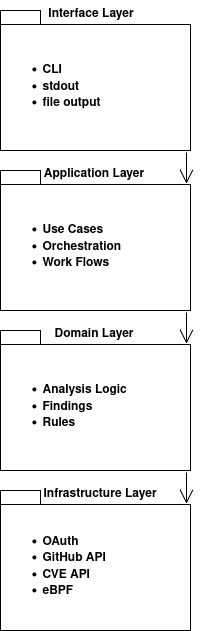
\includegraphics[scale=0.5, keepaspectratio]{images/high-level-layers}
\caption{High Level Layers}
\end{figure}

The Hexagonal Architecture is used to bring the layers to life and substantiate the aspects of each layer.

\subsubsection{Hexagonal Architecture}

The Hexagonal Architecture adheres to the Separation of Concern principle. It is also referred to as the Ports and Adapters architecture. The main goal is to create abstraction layers resulting in isolation of the core business logic and any outside concerns and components(database, external APIs, frameworks etc.).\newline The architecture has an elegant solution for the flow of data. The input of data which can originate from a user or other external service passes into the application at a port using an adapter. The output reverses the flow of data and goes from the application to an apdapter through the port \footnote{Pablo Martinez. Hexagonal Architecture, there are always two sides to every story. [online] homepage: medium.com URL: https://medium.com/ssense-tech/hexagonal-architecture-there-are-always-two-sides-to-every-story-bc0780ed7d9c [Accessed 08.01.2026]}.

\subsection{Component Design}

!

\subsection{UML Diagram}

Maybe Use Case Diagram, Activity Diagram

\subsection{Data Flow}

\subsubsection{Description}

\subsubsection{Flowchart}

\subsection{User Interface Design}

The tool has a command line interface (CLI). The Typer library will be used to build the CLI. The following code shows an outline of the structure:

\subsubsection{CLI Menu}

The CLI has various flags for options to choose from:

\begin{itemize}
	\item -s flag: statical mode for statical analysis
	\item -b flag: behavioral mode for behavioral analysis
	\item -u flag: ultimate mode, for both statical and behavioral analysis
	\item -r flag: generates a report text file of the findings (default output is stdout)
\end{itemize}

\subsection{Security Considerations}

\subsection{Design Decisions and Rationale}

\subsubsection{Hexagonal Architecture}

\footnote{URL: https://dev.to/dyarleniber/hexagonal-architecture-and-clean-architecture-with-examples-48oi}
\footnote{URL: https://senseisrl.it/en/tech-tales/hexagonal-architecture-principles-and-benefits}

\subsection{Limitations}

\subsubsection{Edge Cases}

\subsubsection{Future Improvements}